% Mindmap
% Author: Stefan Kottwitz
% https://www.packtpub.com/hardware-and-creative/latex-cookbook
\documentclass[border = 60pt]{standalone} 
%%%<
\usepackage{verbatim}
\usepackage[slovene]{babel}
\usepackage[utf8]{inputenc}
%%%>
\begin{comment}
:Title: Mindmap
:Tags: Mindmaps;Cookbook
:Author: Stefan Kottwitz
:Slug: mindmap

A mindmap of TeX concepts.
\end{comment}
\usepackage[landscape]{geometry}
\usepackage{tikz}
\usetikzlibrary{mindmap}
\usepackage{metalogo}
\usepackage{dtklogos}
\begin{document}
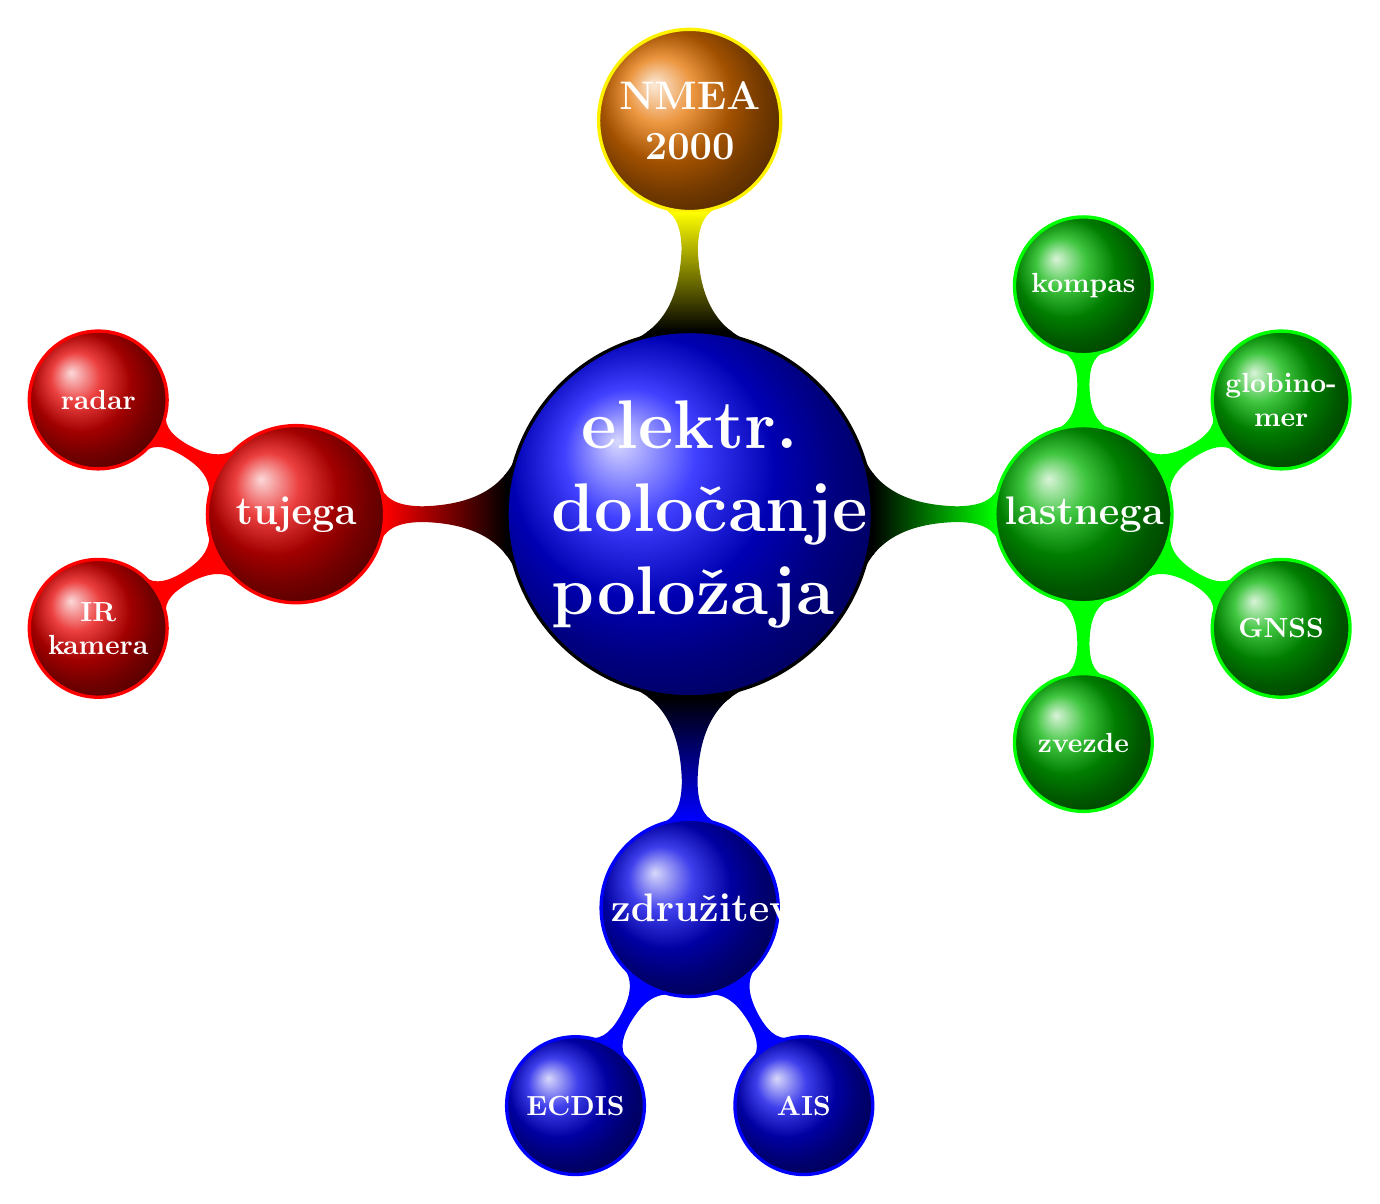
\begin{tikzpicture}
  \path [
    mindmap,
    text = white,
    level 1 concept/.append style =
      {font=\Large\bfseries, sibling angle=90},
    level 2 concept/.append style =
      {font=\normalsize\bfseries},
    level 3 concept/.append style =
      {font=\small\bfseries},
    tex/.style     = {concept, ball color=blue,
      font=\Huge\bfseries},
    lastnega/.style = {concept, ball color=green!70!black},
    pripomocki/.style = {concept, ball color=blue!90!black},
    tujega/.style = {concept, ball color=red!90!black},
    elektronika/.style = {concept, ball color=orange!90!black}
  ]
  node [tex] {elektr. določanje položaja} [clockwise from=0]
    child[concept color=green, nodes={lastnega}] {
      node {lastnega} [clockwise from=90]
        child { node {kompas} }
        child { node {globino-mer} }
        child { node {GNSS} }
        child { node {zvezde} }}
    child [concept color=blue, nodes={pripomocki}] {
      node {združitev} [clockwise from=300]
        child { node {AIS} }
        child { node {ECDIS} }}
    child [concept color=red, nodes={tujega}] {
      node {tujega} [clockwise from=210]
        child { node {IR kamera} [clockwise from=300]}
          %child { node {IR kamera} }}
        child { node {radar} [clockwise from=60]}}
          %child { node {Pro \TeX t} }}}
    child [concept color=yellow, nodes={elektronika}] {
      node {NMEA 2000} };
\end{tikzpicture}
\end{document}